\documentclass[11pt]{beamer}
\usepackage[utf8]{inputenc}
\usepackage[T1]{fontenc}
\usepackage{lmodern}
\usepackage{amsmath}
\usepackage{amsfonts}
\usepackage{amssymb}
\usepackage{graphicx}
\usetheme{Copenhagen}
\begin{document}
    \author{Liu Xuefeng}
    \title{Statistics in Business Analytics}
    %\subtitle{}
    %\logo{}
    %\institute{}
    \date{\today}
    %\subject{}
    %\setbeamercovered{transparent}
    %\setbeamertemplate{navigation symbols}{}
    \begin{frame}[plain]
    \maketitle
\end{frame}

\section{Concepts}
%\subsection{Basic Concepts}
\begin{frame}
\frametitle{Basic Concepts}
    \begin{itemize}
        \item Business analytics is the scientific process of transforming data into insight for making better decisions.
        \item Statistics is a branch of mathematics working with data collection, organization, analysis, interpretation and presentation.
        \item Some examples of business analytics by area: financial analytics, human resource analytis, market analytics, supply chain analytics, sports analytics, web analytics.
    \end{itemize}
\end{frame}

\begin{frame}
\frametitle{Tasks in Business Analytics}
\begin{figure}
    \centering
    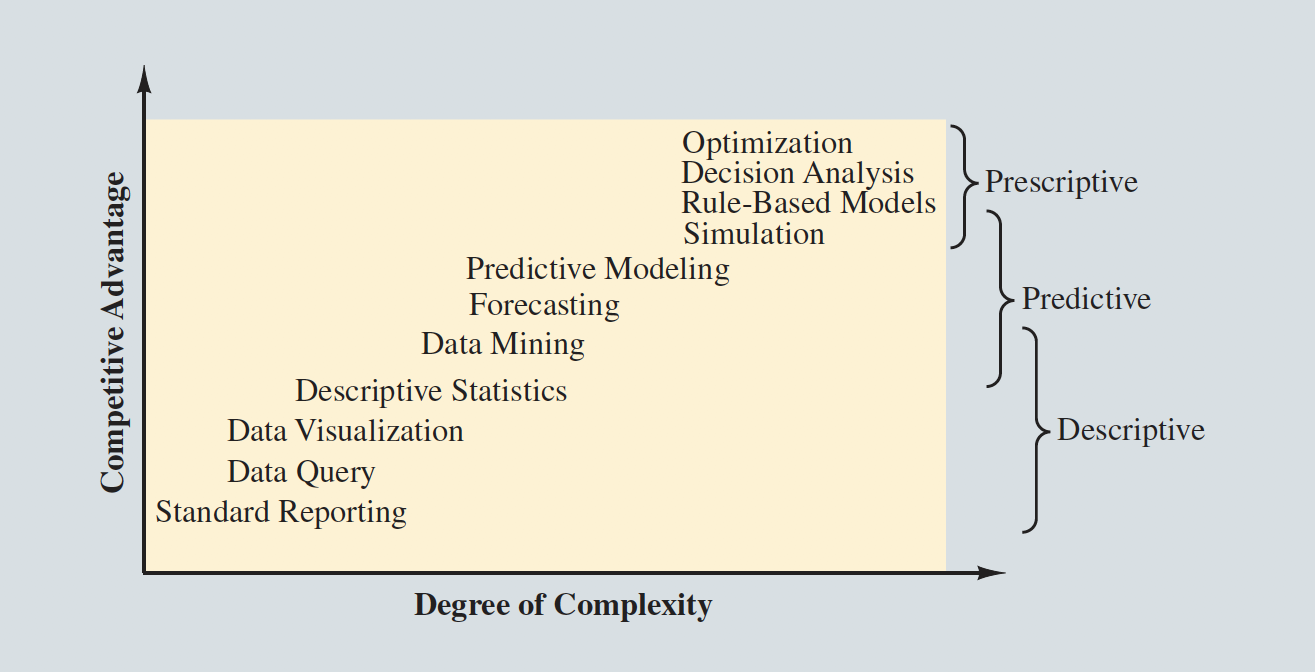
\includegraphics[width=0.9\linewidth]{pic/ba_spectrum}
%    \caption{faefe}
    \label{fig:baspectrum}
\end{figure}

\end{frame}

\begin{frame}
\frametitle{Tasks in Statistics}
    \begin{itemize}
        \item Descriptive Statistics: Analytical tools that describe what has happened.
        \item Data visualization.
        \item Statistical inference: Techniques that use models constructed from past data to ascertain the impact of one variable on another.
        \item Predictive analysis: Techniques that use models constructed from past data to predict the future.
        \item Prescriptive analysis: Techniques that analyze input data and yield a best course of action.
    \end{itemize}

\end{frame}

\section{Descriptive Statistics}

\begin{frame}
\frametitle{Descriptive Statistics}
\begin{itemize}
    \item The role of descriptive analytics is to collect and analyze data to gain a better understanding of variation and its impact on the business setting.
    \item Example of descriptive statistics, mean, standard deviation, TWAP, VWAP.
\end{itemize}
\end{frame}

\begin{frame}
\frametitle{Type of Data}
\begin{itemize}
    \item Quantitative data. Data are considered quantitative data if numeric and arithmetic operations, such as addition, subtraction, multiplication, and division, can be performed on them.
    \item Categorical data. We can summarize categorical data by counting the number of observations or computing the proportions of observations in each category.
\end{itemize}
\end{frame}

\begin{frame}
\frametitle{Measures of Location}
\begin{itemize}
    \item Mean. Excel formula: AVERAGE
    \[\bar{x} = \frac{x_1+x_2+\cdots+x_n}{n}\]
    \item Median: the value in the middle when the data are arranged in ascending order (smallest to largest value). Excel formula: MEDIAN
    \item Mode: the value that occurs most frequently in a data set. Excel formula: MODE.MULT
    \item Geometric mean.Excel formula: GEOMEAN
    $$\bar{x}_g=\sqrt[n]{(x_1)(x_2)\cdots(x_n)}$$
\end{itemize}
\end{frame}

\begin{frame}
\frametitle{Measures of Variability}
\begin{itemize}
    \item Range. The range can be found by subtracting the smallest value from the largest value in a data set.Excel formula: MAX - MIN
    \item Variance. Excel formula: VAR.S
    $$s^2=\frac{\sum_{i=1}^{n}(x_i-\bar{x})^2}{n-1}$$
    \item Standard deviation. Excel formula: STDEV.S
    $$s=\sqrt{s^2}$$
\end{itemize}
\end{frame}

\begin{frame}
\frametitle{Measures of Association between Two Variables}
\begin{itemize}
    \item Covariance is a descriptive measure of the linear association between two variables. Excel formula: COVARIANCE.S
    $$s_{xy}=\frac{\sum_{i=1}^{n}(x_i-\bar{x})(y_i-\bar{y})}{n}$$
    \item Correlation coefficient measures the relationship between two variables. Excel formula: CORREL.
    $$r_{xy}=\frac{s_{xy}}{s_xs_y}$$
\end{itemize}
\end{frame}

\section{Data Visualization}

\begin{frame}
\frametitle{Data Visualization}
\begin{itemize}
    \item Tables
    \item Charts: scatter plot, line plot, bubble plot, heat map, bar chart, pie chart.
\end{itemize}
\end{frame}

\section{Statistical Inference}

\begin{frame}
\frametitle{Hypothesis Tests}
\begin{itemize}
    \item Hypothesis test is the process of making a conjecture about the value of a population parameter, collecting sample data that can be used to assess this conjecture, measuring the strength of the evidence against the conjecture that is provided by the sample, and using these results to draw a conclusion about the conjecture.
    \item Null hypothesis: The hypothesis tentatively assumed to be true in the hypothesis testing procedure. Usually denoted by $H_0$.
    \item Alternative hypothesis: The hypothesis concluded to be true if the null hypothesis is rejected. Usually denoted by $H_a$.
\end{itemize}
\end{frame}

\begin{frame}
\frametitle{Hypothesis Tests}
\begin{itemize}
    \item Type I error: The error of rejecting $H_0$ when it is true.
    \item Type II error: The error of accepting $H_1$ when it is false.
    \item Principal: protect null hypothesis, put what you want to prove as alternative hypothesis.
\end{itemize}
\end{frame}

\begin{frame}
\frametitle{Two-Sample Student's T Test}
\begin{itemize}
    \item Two-sample Student's t test is used to check whether the mean of two populations are the same.
    \item $H_0: \; \mu_1=\mu2$ v.s. $H_a: \; \mu_1 \neq \mu2$
    \item Test statistics: $$t=\frac{\bar{X}_1-\bar{X}_2}{s_p\sqrt{\frac{1}{n_1}+\frac{1}{n_2}}},$$ where 
    $$s_p=\sqrt{\frac{(n_1-1)s^2_{X_1}+(n_2-1)s^2_{X_2}}{n_1+n_2-2}}$$
    \item $t$ follows a T distribution with degree of freedom $n_1+n_2-2$ if $H_0$ holds.
    \item Excel formula: T.TEST.
\end{itemize}
\end{frame}

\section{Predictive Analysis}

\begin{frame}
\frametitle{Simple Linear Regression}
\begin{itemize}
    \item $y=\beta_0+\beta_1x+\epsilon$, where $y$ is response variable, $x$ is explanatory variable, $\beta_0$ is intercept, $\beta_1$ is slope, $\epsilon\sim N(0, \sigma^2)$ is error term.  
\end{itemize}
\end{frame}

\begin{frame}
\frametitle{Butler Trucking Company example}
\begin{figure}
    \centering
    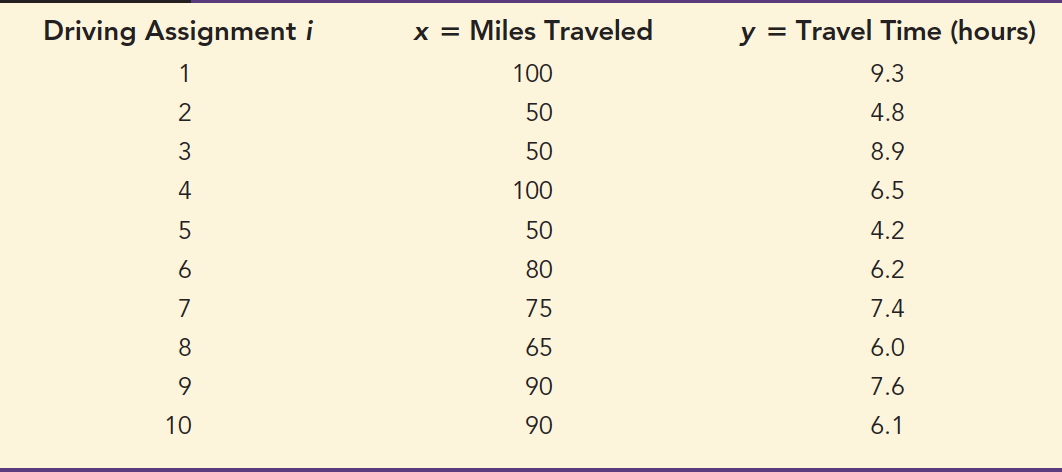
\includegraphics[width=0.6\linewidth]{pic/truck_table}
%    \caption{}
    \label{fig:trucktable}
\end{figure}

\begin{figure}
    \centering
    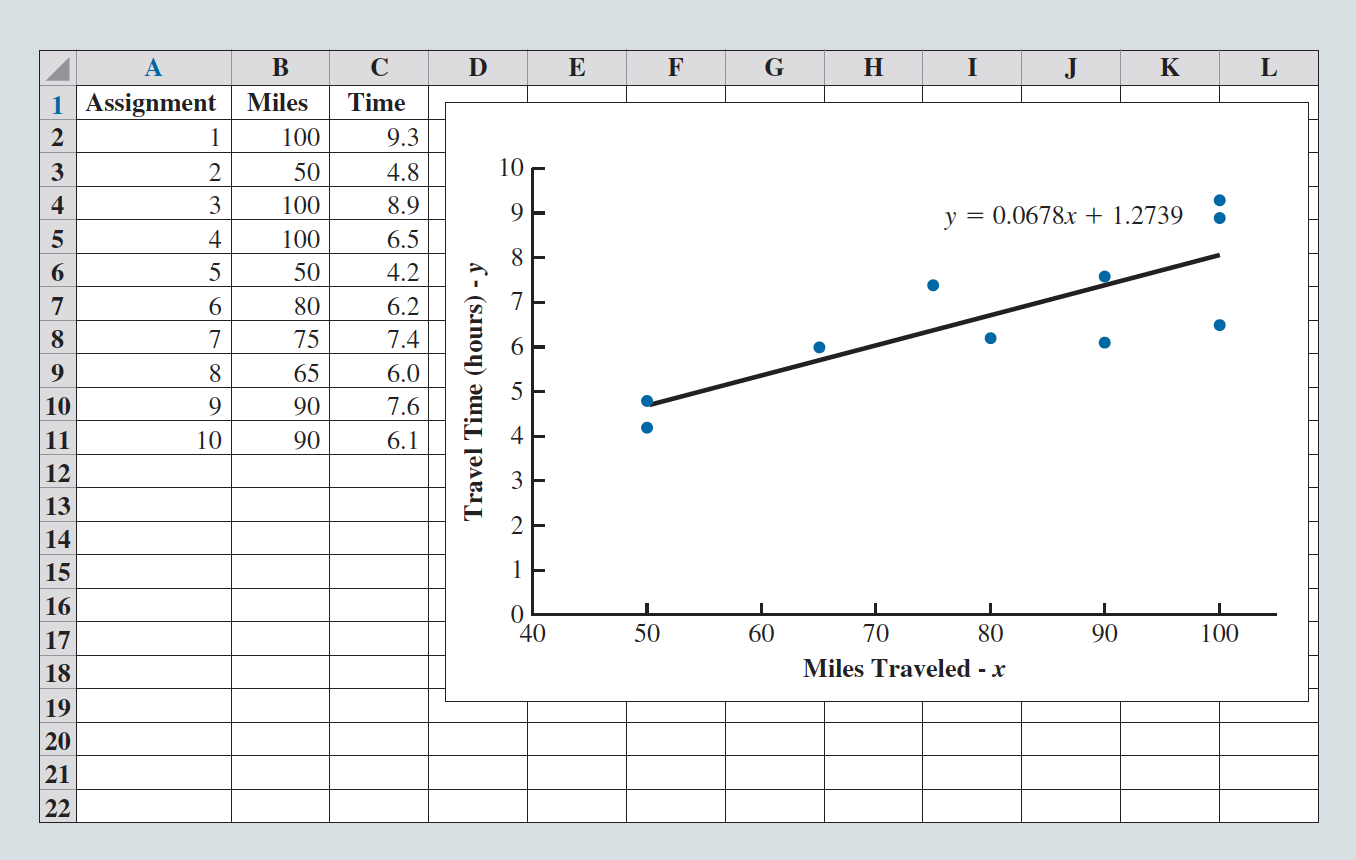
\includegraphics[width=0.6\linewidth]{pic/truck_regression}
%    \caption{}
    \label{fig:truckregression}
\end{figure}

\end{frame}

\begin{frame}
\frametitle{Multiple Linear Regression}
\begin{itemize}
    \item $y=\beta_0+\beta_1x_1+\cdots+\beta_qx_q+\epsilon$.  
    \item Multiple linear regression is an extension to simple linear regression to multiple explanatory variable cases.
\end{itemize}
\end{frame}

\begin{frame}
\frametitle{Generalized Linear Regression}
\begin{itemize}
    \item Generalized linear regression is an extension to multiple linear regression that allows the response variable have distribution other than normal.  
    \item $\eta=\beta_0+\beta_1x_1+\cdots+\beta_qx_q$, where $\eta$ known as link function is an monotonic function of the mean of response variable.
    \item Logistic regression is the most popular generalized linear regression which assumes the response variable follows binary distribution.
\end{itemize}
\end{frame}

\begin{frame}
\frametitle{Logistic Regression Example}

\begin{columns}
    \begin{column}{0.3\textwidth}
        \begin{figure}
            \centering
            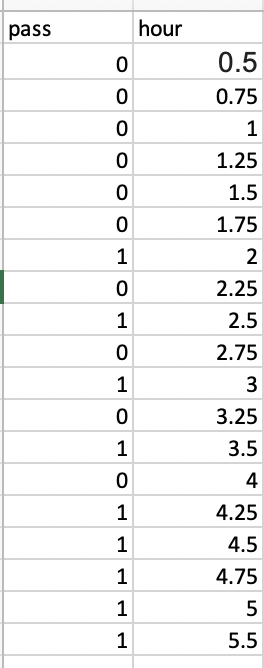
\includegraphics[width=0.7\linewidth]{pic/logistic_data}
            %    \caption{}
            \label{fig:logisticdata}
        \end{figure}
    \end{column}
    \begin{column}{0.7\textwidth}
        \begin{itemize}
            \item In the example, response $y$ is whether a student pass a exam, explanatory variable $x$ is how many hours a student spend on exam preparation.
            \item $$\mu=\frac{1}{1+\exp (-(\beta_0+\beta_1x))}$$, where $\mu=E(y)$ is the probability for a student to pass the exam.
            \item Excel add-in RealStatistics support logistic regression.
        \end{itemize}
    \end{column}
\end{columns}

\end{frame}


\end{document}